\documentclass[aspectratio=169]{beamer}
\usepackage{tikz}
\usetikzlibrary{shadows}
\usepackage{listings}
\usepackage[natbibapa]{apacite}
\makeatletter
\NAT@longnamesfalse
\makeatother

\beamertemplatenavigationsymbolsempty
\setbeamercolor{bluebox}{bg=blue!10}
\newenvironment{colbox}[1][\textwidth]%
  {\begin{beamercolorbox}[wd=#1, rounded=true, shadow=true]{bluebox}}
  {\end{beamercolorbox}}
\setbeamertemplate{footline}{\vskip-6pt\hfill\insertframenumber$\;$\vskip1pt}

\lstdefinestyle{numbers}{language=R,%
  basicstyle=\ttfamily\small\color{blue!50!black},%
  commentstyle=\slshape\color{gray!40!black},%
  numbers=left,numberstyle=\tiny\color{gray!40!black},%
  basewidth={.5em, .4em},%
  showstringspaces=false}

\lstset{language=R,%
  basicstyle=\ttfamily\small\color{blue!50!black},%
%  frame=single,%
  commentstyle=\slshape\color{gray!40!black},%
%  keywordstyle=\bfseries\color{blue!50!black},%
%  identifierstyle=\color{blue!50!black},%
%  stringstyle=\color{green!40!black},%
%  numbers=left,numberstyle=\tiny,%
%  upquote=true,%  straight single quotes for python
  basewidth={.5em, .4em},%
  showstringspaces=false,%
  emphstyle=\color{red}}


\begin{document}

\title{Power Simulation for Logistic Regression}
\author{}
\date{Last modified: 2025-03-02}

\begin{frame}
\thispagestyle{empty}
\titlepage
\end{frame}


\begin{frame}{Overview}

\begin{itemize}
\item Large effects from subtle manipulations?
\begin{itemize}
\item Decision biases from two-hand tapping
\end{itemize}
\item Power simulation for logistic regression
\item Exercises
\end{itemize}

\end{frame}


%%%%%%%%%%%%%%%%%%%%%%%%%%%%%%%%%%%%%%%%%%%%%%%%%%%%%%%%%%%%%%%%%%%%%%%%%%%%%
\section{Large effects from subtle manipulations?}
%%%%%%%%%%%%%%%%%%%%%%%%%%%%%%%%%%%%%%%%%%%%%%%%%%%%%%%%%%%%%%%%%%%%%%%%%%%%%


\begin{frame}{Refresher: Framing}

\begin{itemize}
\item \citet{ TverskyKahneman81}\\[1ex]

``Imagine that the U.S.\ is preparing for the outbreak of an unusual Asian
disease, which is expected to kill 600 people. Two alternative programs to
combat the disease have been proposed'' (p.~453)\\[1ex]

\begin{columns}
\begin{column}{0.4 cm}
\end{column}
%
\begin{column}{5.8 cm}
\begin{colbox}
If Program A is adopted \textbf{200} people will be \textbf{saved} [109]\\[2ex]

If Program B is adopted there is 1/3 probability that \textbf{600} people
will be \textbf{saved}, and 2/3 probability that \textbf{no people} will be
\textbf{saved} [43]
\end{colbox}
\end{column}
%
\begin{column}{5.8 cm}
\begin{colbox}
If Program C is adopted \textbf{400} people will
\textbf{die} [34]\\[2ex]

If Program D is adopted there is 1/3 probability that \textbf{nobody} will
\textbf{die}, and 2/3 probability that\\
\textbf{600} people will \textbf{die} [121]
\end{colbox}
\end{column}
\end{columns}

\vspace{2ex}

\item Odds ratio (OR) $=$ 9.0
\end{itemize}
\end{frame}

% In their classic study of the framing effect, TverskyKahneman81 presented a
% decision dilemma about a new disease. Participants have to decide between
% two options, a safe and a risky option. And, there are two versions of the
% dilemma: In the gain version, you can either gain a certain number of lives
% for sure or you gain everyone's lives with a certain probability (or no
% one's). In the loss version, you loose a number of lives or have the chance
% to loose no one (or everybody). It turned out that participants avoid taking
% the risk under gain framing, but not under loss framing; an indication of
% irrational behavior.


\begin{frame}[fragile]{Decision biases from two-hand tapping}

\begin{itemize}
\item \citet{McElroySeta04}, $n = 48$\\[1ex]

``a behavioral task of finger tapping was used to induce asymmetrical
activation of the respective hemispheres \dots Framing effects were found when
the right hemisphere was selectively activated whereas they were not observed
when the left hemisphere was selectively activated'' (p.~572)

\begin{lstlisting}
     right-hand tapping  left-hand tapping  ratio of odds
     safe risky          safe risky         ratios (ROR)
gain    8     4            12     1
loss    7     4             3     9
OR          1.1                  36         31.5
\end{lstlisting}

\item Our replication \citep[see][]{Gelman20}, $n = 332$
\begin{lstlisting}
gain   52    31            56    27
loss   26    57            30    53
OR          3.7                 3.7          1.0
\end{lstlisting}
\end{itemize}

\end{frame}

% Now, McElroySeta04 wanted to manipulate the framing effect. Here's what they
% did.

% What I want to illustrate here is that given such a subtle manipulation the
% effect is huge. Here is another well-known example.


%%%%%%%%%%%%%%%%%%%%%%%%%%%%%%%%%%%%%%%%%%%%%%%%%%%%%%%%%%%%%%%%%%%%%%%%%%%%%
\section{Examples and exercises}
%%%%%%%%%%%%%%%%%%%%%%%%%%%%%%%%%%%%%%%%%%%%%%%%%%%%%%%%%%%%%%%%%%%%%%%%%%%%%


\begin{frame}{Example: How to fix the two-hand tapping study?}

  {\bf Power simulation\\[2ex]}

  Let us go through the general steps\\[2ex]
\begin{colbox}
\begin{enumerate}
  \item Specify the model including the effect of interest
  \item Generate observations from the model
  \item Test H$_0$
  \item Repeat
\end{enumerate}
\end{colbox}
\end{frame}


\begin{frame}{Example: How to fix the two-hand tapping study?}
  {1. Specify model}
  \begin{itemize}
    \item Logit model with interaction
  \[
  \log \frac{p}{1 - p} = \beta_0
                  + \beta_1 \cdot \text{left hand}
                  + \beta_2 \cdot \text{gain}
                  + \beta_3 \cdot (\text{left hand} \times \text{gain})
\]
    \item Suggest a minimum relevant effect
      \begin{itemize}
        \item We can look at the original framing effect study and its many replications
        \item Former study by \citet{McElroySeta03} found ROR $= 3.4$ for
          similar manipulation
        \item Other studies investigating influencing factors
        \citep[with RORs $\approx$ 2--3, e.\,g., foreign language
      effect,][]{CostaFoucart14, Wickelmaier15}
        %\item Other theoretical assumptions?
      \end{itemize}
    \item Underlying distribution: $X \sim Binom(n, p)$
  \end{itemize}
\end{frame}

% Some background
% 
% Original framing effect \citep{TverskyKahneman81}
% - Odds for safe choice: about 2:1 in gain frame vs.\ 1:2 in loss frame
% - OR approx 4
% 
% Manipulation of framing effect
% - Foreign-language effect \citep{CostaFoucart14, Wickelmaier15}:
%   ROR approx 2-3
% 
% Suggesting a minimum relevant effect
% 
% With right-hand tapping, framing effect is halved
% - OR $=$ 2, $\sqrt{2}$:1 vs.\ 1:$\sqrt{2}$
% 
% With left-hand tapping, framing effect is doubled
% - OR $=$ 8, $\sqrt{8}$:1 vs.\ 1:$\sqrt{8}$
% 
% ROR = 4
% 
% log(1:sqrt(2))
% log(1/2)
% log(2)
% log(4)


\begin{frame}{Example: How to fix the two-hand tapping study?}
  {1. Specify model}
\begin{columns}
\begin{column}{8cm}
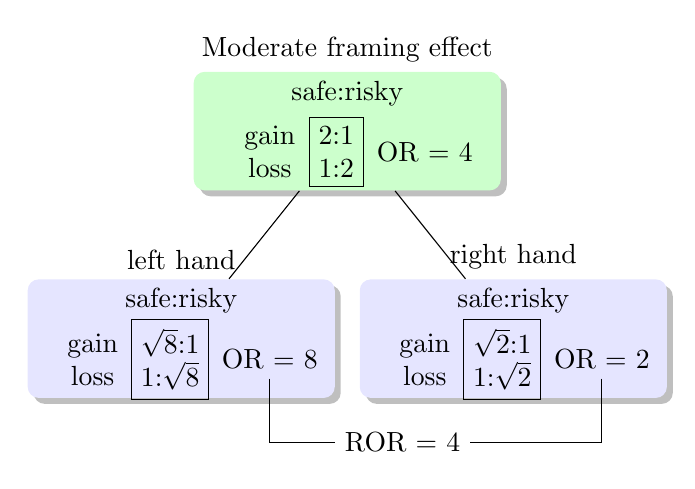
\begin{tikzpicture}
[x=40, y=25,
 every node/.style={align=center},
 nodeOut/.style={fill=blue!10, rounded corners, minimum width=3.9cm,
   drop shadow},
 nodeOR/.style={draw}
]
\node[nodeOut, fill=green!20,
  label={Moderate framing effect}] (O1) at ( 0,  4.3) {safe:risky\\[4ex]};
\node                at (-0.7, 4)  {gain\\ loss};
\node[nodeOR]        at (-0.1, 4) {2:1\\ 1:2};
\node                at ( 0.7, 4) {OR $=$ 4};
\node[nodeOut, label={left hand}] (O2) at (-1.5, 1.3) {safe:risky\\[4ex]};
\node                at (-2.3, 1)  {gain\\ loss};
\node[nodeOR]        at (-1.6, 1) {$\sqrt{8}$:1\\ 1:$\sqrt{8}$};
\node           (R8) at (-0.7, 1) {OR $=$ 8};
\node[nodeOut, label={right hand}] (O3) at ( 1.5, 1.3) {safe:risky\\[4ex]};
\node                at ( 0.7, 1)  {gain\\ loss};
\node[nodeOR]        at ( 1.4, 1) {$\sqrt{2}$:1\\ 1:$\sqrt{2}$};
\node           (R2) at ( 2.3, 1) {OR $=$ 2};
\node           (O4) at (0.5, -0.2) {ROR $=$ 4};
\draw (O1) -- (O2);
\draw (O1) -- (O3);
\draw (R8) -- (-0.7, -0.2) -- (O4);
\draw (R2) -- ( 2.3, -0.2) -- (O4);
\end{tikzpicture}
\end{column}
\begin{column}{6cm}
  Translating into parameters
  \begin{itemize}
    \item $\exp(\beta_0) = \frac{1}{\sqrt{2}}$\\
      odds in reference categories: right and loss
    \item $\exp(\beta_1) = \frac{1}{2}$\\
      OR of switching to left hand
    \item $\exp(\beta_2) = 2$\\
      OR of switching to gain frame
    \item $\exp(\beta_3) = 4$\\
      ROR
  \end{itemize}
\end{column}
\end{columns}
\vfill
\[
  \log \frac{p}{1 - p} = \beta_0
                  + \beta_1 \cdot \text{left hand}
                  + \beta_2 \cdot \text{gain}
                  + \beta_3 \cdot (\text{left hand} \times \text{gain})
\]

\end{frame}


\begin{frame}[fragile]{Example: How to fix the two-hand tapping study?}
  {2. Generate observations}
  \begin{itemize}
    \item Calculate logits for the model
\begin{lstlisting}
dat <- read.table(header = TRUE, text = "
  hand frame
     r  gain
     r  loss
     l  gain
     l  loss")                                          # ref. cat.
dat$hand <- factor(dat$hand, levels = c("r", "l"))          #   right
dat$frame <- factor(dat$frame, levels = c("loss", "gain"))  #   loss

expbeta <- c(1/sqrt(2), 1/2, 2, 4)  # ROR = 4, linear on logit scale
logit <- model.matrix(~ hand * frame, dat) %*% log(expbeta)
\end{lstlisting}
  \end{itemize}
\end{frame}


\begin{frame}[fragile]{Example: How to fix the two-hand tapping study?}
  {2. Generate observations}
  \begin{itemize}
    \item Simulate data from binomial distribution
\begin{lstlisting}
n <- 100
y <- rbinom(4, size = n/4, prob = plogis(logit))

## Sim 1             Sim 2             ...
## hand frame  y     hand frame  y
##    r  gain  16       r  gain  15
##    r  loss  7        r  loss  13
##    l  gain  21       l  gain  19
##    l  loss  9        l  loss  7
\end{lstlisting}
  \end{itemize}
\end{frame}


\begin{frame}[fragile]{Example: How to fix the two-hand tapping study?}
  {3. Test H$_0$}
  \begin{itemize}
    \item Fit null model to your generated observations, H$_0$: $
      \beta_3 = 0$
\begin{lstlisting}
m1 <- glm(cbind(y, n/4 - y) ~ hand + frame, binomial, dat)
\end{lstlisting}
    \item Fit interaction model to your generated observations, H$_1$:
      $\beta_3 \neq 0$
\begin{lstlisting}
m2 <- glm(cbind(y, n/4 - y) ~ hand * frame, binomial, dat)
## ROR estimate = 5.9
\end{lstlisting}
    \item Perform a likelihood ratio test of the interaction
\begin{lstlisting}
anova(m1, m2, test = "LRT")
## Analysis of Deviance Table
## 
## Model 1: cbind(y, n/4 - y) ~ hand + frame
## Model 2: cbind(y, n/4 - y) ~ hand * frame
##   Resid. Df Resid. Dev Df Deviance Pr(>Chi)  
## 1         1     4.3436                       
## 2         0     0.0000  1   4.3436  0.03715
\end{lstlisting}
  \end{itemize}
\end{frame}


\begin{frame}[fragile]{Example: How to fix the two-hand tapping study?}
  {4. Repeat}
\begin{itemize}
\item Do previous steps repeatedly\\
-- Calculate the proportion of significant tests ($=$ power)\\
-- Adjust $n$ to reach the preset power criterion
\end{itemize}
\end{frame}


% \begin{frame}{Exercises}
% 
% Reanalyze the original data
% \begin{itemize}
% \item Read the original data \citep{McElroySeta04} into R.\\
%       Hint: Mind the order of the factor levels
% \item Use \texttt{glm()} to fit a logistic regression model
% \item Formulate H$_0$ in terms of the model parameters\\
%       Which parameter represents the ratio of odds ratios (ROR)?
% \item Test the interaction between hand and frame
% \item Interpret the results of the test\\[2ex]
% \end{itemize}
% 
% Redo the analysis for the replication data
% \end{frame}


% \begin{frame}{Exercises}
% 
% Logit model with interaction (two-hand tapping)
% 
% \begin{itemize}
% \item Specify the model
% \item Parameter recovery\\
% -- Fix the parameters to the values determined before, simulate,
% recover\\[1ex]
% 
% \item Power simulation\\
% -- Calculate the sample size necessary to detect the effect\\[2ex]
% \end{itemize}
% 
% Simple logit model (framing effect only)
% 
% \begin{itemize}
% \item Specify the model
% \item Parameter recovery
% \item Power simulation\\
% -- Draw a power curve for (at least) three different $n$ values
% \end{itemize}
% \end{frame}


%%%%%%%%%%%%%%%%%%%%%%%%%%%%%%%%%%%%%%%%%%%%%%%%%%%%%%%%%%%%%%%%%%%%%%%%%%%%%


\begin{frame}{References}
\renewcommand{\bibfont}{\footnotesize}
\bibliographystyle{apacite}
\bibliography{../lit}
\end{frame}

\end{document}

